\subsection{Collaboration}
\subsubsection{Groups}
Permissions may also be assigned to a list of users via groups. These groups will allow sets of users to share data together openly. The group will be controlled by an admin. This administrative position will have rights to add and delete users from the group. Along with the permission to move users around, the admin may also set the shared access rights for the group. Certain individuals or organizations may want to allow access to groups of people. Instead of having to give permissions to each person, a user or organization may allow a set of users to see their data. This will allow for organizations, such as universities, to share with other organizations quickly. This will reduce the stress of having to remove and add new users as they cycle out of foreign organizations.

\begin{figure}[t]
  \begin{center}
  \captionsetup{width=.8\linewidth}
  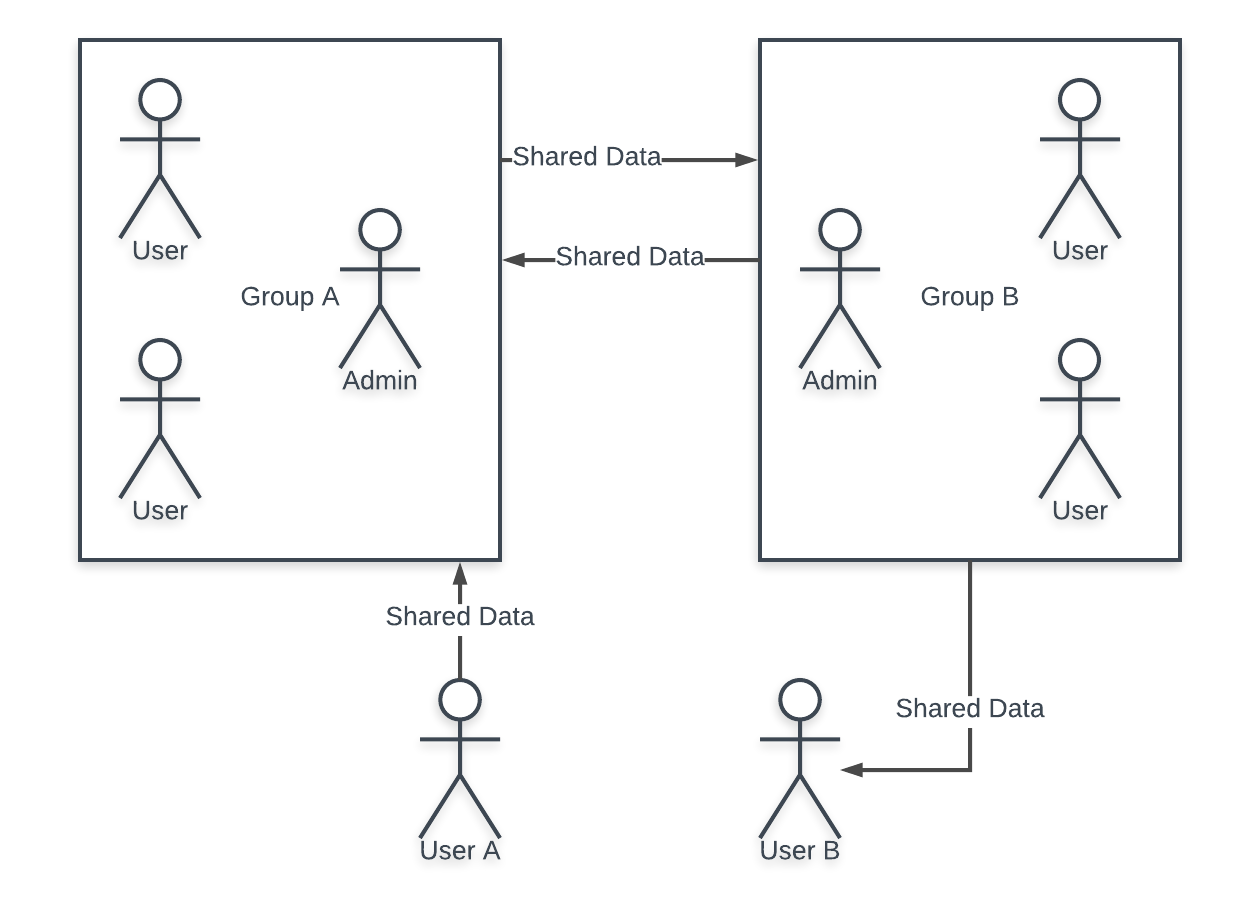
\includegraphics[width=0.8\linewidth]{DataPermissions}
  \caption{All users of Group A have permissions to User A\textquotesingle s data; All Users from Group A have access to the data of Group B and vice versa; User B Has rights to Group B\textquotesingle s Data; No group or user has access to User B\textquotesingle s data}
  \end{center}
\end{figure}

\subsubsection{Access Rights}
Users and groups may set two types of access rights to their files. The first being open and the second being restricted. As the name suggests, open files are open to the public. No special permission is required in order to access them. Thus, any user of our application may go to wherever they are hosted and pull them onto their own machine. If a user or group decides that they do not wish to have their files or data open to the world, then they may choose the restricted option. This option only allows certain users or groups to have access to the files or data. The specific rights are given as follows.\par
Users and groups may have different levels of permission given to them, refered to as access rights. These access rights can come in two forms: the right to read and the right to edit. The right to read allows a user or group to view the data the a user has published on the application and to download the files from the host machine onto their local machine. The right to edit allows users or groups to run analysis on data and use the tools we provide on the files or data. From that point forward, whatever the local user does with the data is beyond the control of either us or anyone affiliated with our program.
